\let\negmedspace\undefined
\let\negthickspace\undefined
\documentclass[journal]{IEEEtran}
\usepackage[a5paper, margin=10mm, onecolumn]{geometry}
\usepackage{lmodern} % Ensure lmodern is loaded for pdflatex
\usepackage{tfrupee} % Include tfrupee package

\setlength{\headheight}{1cm} % Set the height of the header box
\setlength{\headsep}{0mm}     % Set the distance between the header box and the top of the text

\usepackage{gvv-book}
\usepackage{gvv}
\usepackage{cite}
\usepackage{amsmath,amssymb,amsfonts,amsthm}
\usepackage{algorithmic}
\usepackage{graphicx}
\graphicspath{{./figs/}}
\usepackage{textcomp}
\usepackage{xcolor}
\usepackage{txfonts}
\usepackage{listings}
\usepackage{enumitem}
\usepackage{mathtools}
\usepackage{gensymb}
\usepackage{comment}
\usepackage[breaklinks=true]{hyperref}
\usepackage{tkz-euclide} 
\usepackage{listings}
\usepackage{gvv}                                        
\def\inputGnumericTable{}                                 
\usepackage[latin1]{inputenc}                                
\usepackage{color}                                            
\usepackage{array}                                            
\usepackage{longtable}                                       
\usepackage{calc}                                             
\usepackage{multirow}                                         
\usepackage{hhline}                                           
\usepackage{ifthen}                                           
\usepackage{lscape}
\usepackage{circuitikz}
\tikzstyle{block} = [rectangle, draw, fill=blue!20, 
text width=4em, text centered, rounded corners, minimum height=3em]
\tikzstyle{sum} = [draw, fill=blue!10, circle, minimum size=1cm, node distance=1.5cm]
\tikzstyle{input} = [coordinate]
\tikzstyle{output} = [coordinate]


\begin{document}
	
	\bibliographystyle{IEEEtran}
	\vspace{3cm}
	
	\title{1.5.29}
	\author{EE25BTECH11042 - Nipun Dasari}
	\maketitle
	% \newpage
	% \bigskip
	{\let\newpage\relax\maketitle}
	
	\renewcommand{\thefigure}{\theenumi}
	\renewcommand{\thetable}{\theenumi}
	\setlength{\intextsep}{10pt} % Space between text and floats
	
	
	\numberwithin{equation}{enumi}
	\numberwithin{figure}{enumi}
	\renewcommand{\thetable}{\theenumi}
	
	\textbf{Question}:\\
	The coordinates of the point P dividing the line segment joining the points A (1, 3)
	and B (4, 6), in the ratio 2 : 1 are \\ 
	\solution \\
	According to the question, \\
	Consider the coordinate as following vectors \\ 

	Given the points A and B
	
	\begin{align*}
		\vec{A} = \begin{myvec}{1\\3} \end{myvec} , \vec{B} = \begin{myvec}{4\\6} \end{myvec}
	\end{align*}
	\textbf{The formula for internal division of vectors is where $\vec{P}$ divides $\vec{A}$ and $\vec{B}$ in the ratio k:1}
	\begin{align*}
	\vec{P} =	\frac{k\vec{B} + \vec{A}}{1+k} 
	\end{align*}
	Thus by formula
	\begin{align*}
	\vec{P} = \frac{1}{1+2}\brak{\begin{myvec}{1\\3} \end{myvec}+2\begin{myvec}{4\\6} \end{myvec}}
	\end{align*}
	\begin{align*}
		\vec{P} = \frac{1}{3}\brak{\begin{myvec}{1\\3} \end{myvec}+\begin{myvec}{8\\12} \end{myvec}}
	\end{align*}
	\begin{align*}
		\vec{P} = \frac{1}{3}\begin{myvec}{9\\15}\end{myvec}
	\end{align*}
	\begin{align*}
	\therefore	\vec{P} = \begin{myvec}{3\\5}\end{myvec}
	\end{align*}

\begin{figure}[H]
	\centering
	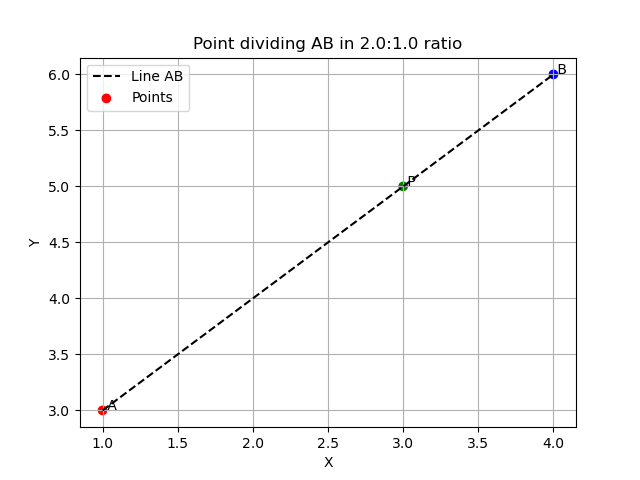
\includegraphics[width = 0.8\columnwidth]{q1.1.png}
	\caption*{}
	\label{q1.1}
\end{figure}

\begin{figure}[H]
	\centering
	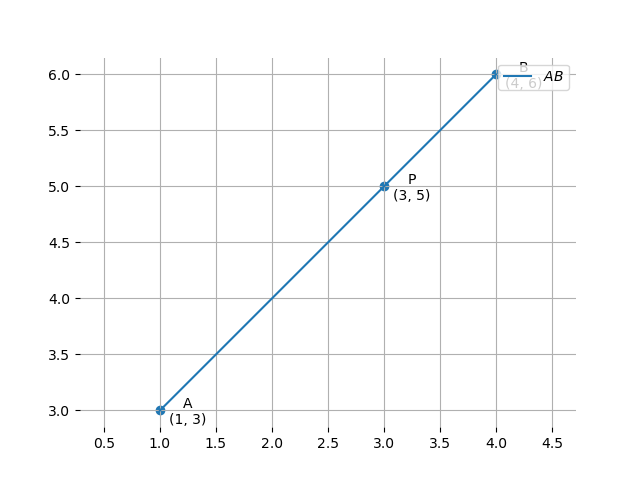
\includegraphics[width = 0.8\columnwidth]{q1.2.png}
	\caption*{}
	\label{q1.2}
\end{figure}

\end{document}
	
	
	